\documentclass[review]{elsarticle}
%\documentclass[final,times,letterpaper,12pt]{elsarticle}

\usepackage{lineno,hyperref}
\usepackage{graphicx} 
\usepackage{subcaption}
\usepackage{amsmath}
\usepackage{booktabs}


\usepackage[dvipsnames]{xcolor} % Für Einfärbung von Notizen. Sollte am Ende wieder entfernt werden.

\modulolinenumbers[5]

%\usepackage{etoolbox}
% \patchcmd{<cmd>}{<search>}{<replace>}{<success>}{<failure>}
%\patchcmd{\emailauthor}{(#2)}{}{}{}
\patchcmd{\urlauthor}{(#2)}{}{}{}

\journal{Journal of PLACEHOLDER}


%%%%%%%%%%%%%%%%%%%%%%%
%% Elsevier bibliography styles
%%%%%%%%%%%%%%%%%%%%%%%
%% To change the style, put a % in front of the second line of the current style and
%% remove the % from the second line of the style you would like to use.
%%%%%%%%%%%%%%%%%%%%%%%

%% Numbered
%\bibliographystyle{model1-num-names}

%% Numbered without titles
%\bibliographystyle{model1a-num-names}

%% Harvard
%\bibliographystyle{model2-names.bst}\biboptions{authoryear}

%% Vancouver numbered
%\usepackage{numcompress}\bibliographystyle{model3-num-names}

%% Vancouver name/year
%\usepackage{numcompress}\bibliographystyle{model4-names}\biboptions{authoryear}

%% APA style
\bibliographystyle{model5-names}
\biboptions{authoryear}

%% AMA style
%\usepackage{numcompress}\bibliographystyle{model6-num-names}

%% `Elsevier LaTeX' style
%\bibliographystyle{elsarticle-num}
%%%%%%%%%%%%%%%%%%%%%%%

\begin{document}

\begin{frontmatter}

\title{PLACEHOLDER Title}

\author {Jasper Bär\corref{cor1}}
\ead{ja.baer@stat-econ.uni-kiel.de}
\ead[url]{PLACEHOLDER Github url}

\cortext[cor1]{PLACEHOLDER}

\begin{abstract}
PLACEHOLDER Abstract
\end{abstract}

\begin{keyword}
PLACEHOLDER Keyword 1 \sep Keyword 2 \sep Keyword 3 \sep Keyword 4 \sep Keyword 5
\end{keyword}

\newpageafter{abstract}

\end{frontmatter}

\newpage

\section{Introduction} \label{sec:intro}

%Hook/Attention-grabber (existiert)
%Background and context (existiert, aber noch lückenhaft und muss besser zusammengefügt werden)
%Gap in the literature (existiert, anders in den Text einfügen?)
%Research question or objective (existiert)
%Scope and limitations (fehlt noch)
%Methodological approach (existiert)
%Significance and contribution (existiert)
%Roadmap/Outline (wegglassen?)

% Hook 
Central bank communication has become a vital instrument in modern monetary policy \citep{Blinderetal2017}. Central banks use communication as a tool for guiding inflation expectations and ensuring trust in their monetary policy. Historically, much of this communication has been directed towards financial experts. However, in recent years, central banks have increasingly been reaching out to the general public \citep{Blinderetal2022}. The media plays a critical role in this process by disseminating central bank communication to a broader audience. Therefore, it is essential to understand how the media reports on central bank communication to analyze the impact of central bank communication on the general public.
%
% Background and context
%
% Literature on inflation expectations
% Literature on Media impact on expectations
%
\\
Since \cite{Carroll2003} created a model for inflation expectations that considers the amount of media coverage several studies have analyzed the role of media coverage for the inflation expectation forming process. \cite{Draeger2015} find a small effect of media on inflation expectations and perception for Sweden. Similar, \cite{LamlaLein2014} find that media reporting report the accuracy of German household inflation expectations. \citep{Larsen2021} show that the news topics also have predictive power inflation expectation. \cite{Ehrmann2017} show that increased media coverage leads to the strongest improvements in inflation expectations accuracy during recessions and for individuals with pessimistic views or financial difficulties.  
%\cite{Jansen2018} however find that more freuqent readership of popular newspapers is assoziated the less inflation perception accuracy for Dutch households. 
%
% Literature on central banks impact on household inflation
%
\\
% "Fed speak on main street: Central bank communication and
% household expectations" has good literature overview for this section.
%
Another recent branch of the literature investigates the impact of central bank communication on household inflation expectations. \cite{Coibion2022} show that the Fed's communication can have a significant effect on the households inflation expectations when the communication is directly presented to the households. However, the effect of the communication is significantly damped when the same information is presented in the form of newspaper articles. This view is in line with \cite{Gardt2022} who demonstrate that households mostly hear about the ECB's monetary policy through television and newspapers (online and printed) and rarely by using direct sources like the ECB website. Similar, \cite{LamalaVinogradov2019} find that FOMC announcements have no impact on consumers' inflation perception and expectation, but that FOMC announcements increase the probability of consumers to receive news about the FOMC announcements. 
%
% Literature on Central banks in media
%
\\
Several studies investigate how central bank communication is perceived by the media \cite{Berger2011} and \cite{Picaultetal2022} show that the medias assessment of ECB policy decision is highly responsive to the content of ECB press conferences. %More citations?
%
% Gap in the literature
%
\\
Similar to \cite{Picaultetal2022}, I adopt a framework proposed by \cite{HayoNeuenkirch2015} where the media acts as a channel between central bank communication and the perception of monetary policy by financial markets. Following \cite{Nimark2019} who formalize that agents delegate their information choice to the media rather than monitor all relevant events themselves. Hence, news act as a channel between through which households receive information about the central bank communication. Building on these two frameworks, I assume that the media coverage of central bank communication acts as a channel between the central bank and households. I assume that households consume the news from the media about the central bank communication rather than directly from the central bank communication itself. 
%
%This view gets supported by a number of survey-based studies indicating that household are often poorly informed about monetary policy and the objectives of their respective central banks. \cite{Cruijsenetal2015} show that Dutch households understanding about the ECB's objectives are poor. Similar most German \citep{HayoNeuenkirch2018} and Italian \citep{Bottonetal2021} households do not know that the main objective of the ECB is to maintain price stability in the euro zone. However, \cite{Cruijsenetal2015} and \cite{HayoNeuenkirch2018} show that people who receive their information about monetary policy via television and newspapers are better informed their central bank and monetary policy.\textcolor{red}{(To close to Blinder et al. 2022)}
%
% Research Question
%
\\
I am examining the impact of media coverage in newspapers on households' inflation expectation accuracy, specifically focusing on reporting of ECB press conferences and news about inflation. Firstly, I explore whether the inflation information presented in newspapers deviates from the inflation information in the press conferences by the ECB. Secondly, I investigate the extent to which the deviation of inflation information in media coverage and ECB press conferences contributes to explaining the errors in households' inflation expectations.
%
% Scope and limitations
%
%The newspaper data consists of over 6 million German articles ranging from the 1. January of 2002, the day of the introduction of Euro banknotes and coins in Germany, until 31. of December 2018\footnote{The Euro was already introduced as book money in Germany on 1. January 1999.}. The ECB press conference are publicaly available on the official ECB website.
%\\
%
% Significance and contribution
%
\\
This paper is, to my knowledge, the first to explicitly investigate the link between central bank communication and news coverage concerning household inflation expectations. Furthermore, it contributes to the literature by demonstrating how news about inflation deviates from the corresponding ECB communication, allowing for a better understanding of how central bank communication is conveyed to the general public and explaining the channel through which the general public reacts to central bank communication.
%
%Methodological approach
%
\\
I built on the Bayesian learning model \citep{LamlaLein2014} to examine the impact of the difference between inflation related information in media reporting and ECB press conferences on households inflation expectations accuracy. To quantify the inflation related information in the ECB press conferences and news, I apply the lexicon driven procedure by \cite{PicaultRenault2017} to create lexicons for inflation related information for the news and for the ECB press conferences. To measure how closely the media follows ECB press conferences in their news I apply a similar procedure like\cite{Picaultetal2022} and use dependency parsing to identify the grammatical structure of a text and filter out the share of news that reproduce ECB press conferences from general news about inflation. This allow me to measure how closely the media reporting follows the ECB' press conferences.
%
% Teaser Results
%
\\
I find that inflation information in the news and ECB press conferences is strongly correlated with the current inflation in Germany. Furthermore, the the difference inflation reporting in news and ECB press conferences is strongly correlated with the inflation expectation gap between German households and professional inflation forecasts. 
%nochmal nachprüfen
%However, \cite{Picaultetal2022} and \cite{Cruijsenetal2015} note that the perception of financial markets is simultaneously influenced by the central bank communication and the media coverage of the corresponding events and central bank communication.
%A small but rapidly growing branch of the literature focuses on central bank communication, i.e., the information provided by central banks to the general public, and its connection to different variables of interest like financial variables or future monetary decisions of the central bank. For example, \cite{PicaultRenault2017} show that ECB press statements can be used to predict future ECB monetary decisions. \textcolor{red}{(Give more examples)}
%A subbranch of this literature focuses on the connection between inflation expectations and central bank communication. \cite{Picaultetal2022} investigate how the reporting about the ECB in the media can be used to predict financial market inflation expectations. \\
% Kurzer Abschnitt in der ich auf Media Biases eingehe (Media reacts to central bank communication, negativity bias)
\section{Model}\label{sec:Model} 
I augment the Bayesian learning model for inflation expectation by \cite{LamlaLein2014} by explicitly adding a channel for central banks communication. I assume that the central bank sends a noisy signal for the future inflation $\pi_{t+1}$ based on the observation to the media. Let $c_t$ denote the signal that captures inflation-related information about the central bank's inflation forecast $\Theta_t$ that the central bank communicates to the media, i.e., inflation-related information in press conferences. I further assume that the signal is normally distributed $c_t \sim N(\Theta_t, \sigma^c_t)$ with variance $\sigma^c_t$. This assumption also implies that the central bank only sends one unambiguous signal at each period $t$ rather than multiple conflicting signal at the same period.
% In the case of the ECB this inflation forecast is equal to the ECB staff's inflation projection 
%\\
%$ c_t = \pi_{t+1} + \epsilon_t \quad \epsilon_t \sim N(0, \sigma^c_t)$
%\\ 
%where $\epsilon_t$ represents the noise in the central bank's observation. 
%\\
Without the central bank's communication, the media sends a noisy "baseline" signal about the rational forecast of inflation $\Psi_t$ to the households based on a number of media reports $V$ with $s^b_{\nu,t} \sim N(\Psi_t + \alpha_t, \sigma^{sb}_t) $ 
%\\
%$ s^b_t = \alpha_t + \pi_{t+1} + \omega_t  \quad \omega_t \sim N(0, \sigma_t^{s^b}) $
%\\
where $\alpha_t$ captures the media bias. %\footnote{Note that media bias in this context is a rather broad concept and can capture different factors such as political biases or misinformation. For an in depth discussion of the term see (CITE).}. 
The media can decide how closely to follow the central bank's communication. Hence, the media's inflation signal can be defined as 
\begin{equation}
s_{\nu,t} = (1-\lambda_{\nu,t}) s^b_{\nu,t} + \lambda_{\nu,t} c_t \quad 0\leq \lambda_{\nu,t} \leq 1
\end{equation}
where $\lambda_{\nu, t}$ denotes the weight that the media report places on the central bank's signal $c_t$ relative to the "baseline" media signal $s^b_{\nu,t}$. $\lambda_{\nu,t} = 0$ would indicate that the media report ignores the central bank's communication completely while $\lambda_{\nu,t} = 1$ would describe a situation in which the media only reproduces the information from the central bank's communication. 
\\
Given that $s_{\nu,t}$ is a linear combination of normal random variables and assuming that
$\sigma^c_t$ and $\sigma^{sb}_{\nu,t}$ are independent, the media sends a normally distributed signal about $\pi_{t+1}$ with $s_{\nu,t} \sim N(\mu_s, \sigma^s_{\nu,t})$ where 
\begin{equation} 
\mu_{\nu,t}^s = (1-\lambda_{\nu,t}) (\alpha_t + \Psi_t) + \lambda_{\nu,t} \Theta_t 
\end{equation}
\begin{equation}
\sigma_{\nu,t}^s = \lambda_{\nu,t}^2 \sigma_{\nu,t}^{s^b} + (1- \lambda_{\nu,t})^2 \sigma^c_{\nu,t}
\end{equation}
%\begin{equation}
%\mu_s = \lambda_t \alpha_t + \pi_{t+1} 
%\end{equation}
\\
The households hold a prior belief $\gamma_t \sim N(\pi_t, \sigma^h_t)$ about the future inflation $\pi_{t+1}$. Hence, the representative household forms its inflation expectations according to
%\begin{equation}
%f(\pi_{t+1}|c_t, \pi_t, \lambda_{\nu,t}, \alpha_{\nu,t}) \propto \Pi^V_{\nu = 1} h(s_{\nu,t}|\alpha_{\nu,t}, \pi_t, \lambda_{\nu,t}) k(\pi_t)
%\end{equation}
\begin{equation}
f(\pi_{t+1}|s_{\nu,t}) \propto \Pi^V_{\nu = 1} h(s_{\nu,t}|\alpha_t, \pi_t, \lambda_{\nu,t}, c_t) k(\pi_t)
\end{equation}
where $f(.)$ is the posterior belief of a representative household on inflation $\pi_{t+1}$ after receiving the inflation related news signal. Assuming normality the posterior distribution is a normal distribution with mean $\mu_t$
\begin{equation}
\mu_t = \rho_t \pi_t + (1- \rho_t) \bar{\mu_t^s} 
\end{equation}
where
\begin{equation}
\bar{\mu_t^s} = V^{-1} \sum^V_{\nu = 1} \mu_{\nu,t}^s = V^{-1} \sum^V_{\nu =1} (1-\lambda_{\nu,t}) (\alpha_t + \Psi_t) + V^{-1} \sum^V_{\nu =1} \lambda_{\nu,t} \Theta_t  
\end{equation}
\begin{equation}
=\Psi_t + \alpha_t - \bar{\lambda_t} \alpha_t - \bar{\lambda_t} \Psi_t + \bar{\lambda_t}\Theta_t 
\end{equation}
\begin{equation}
=\bar{\lambda_t}(\Theta_t - \Psi_t) + \Psi_t+ \alpha_t(1- \bar{\lambda_t})
\end{equation}
and
\begin{equation}
\rho_t = \frac{\frac{1}{V}\sigma^s_t}{{\sigma^h_t + \frac{1}{V}}\sigma^s_t}
\end{equation}
\\
For $\bar{\lambda_t} = 0$ the mean would be $\mu_t = \rho_t \pi_t + (1- \rho) (\Psi_t +\alpha_t)$. Hence, if the media completely ignores the central bank communication, the mean of the posterior is the weighted average of the prior and the biased media signal\footnote{This case is equivalent to the model from \cite{LamlaLein2014} with media bias.}. If the media perfectly reproduce the central bank communication, i.e, $\bar{\lambda_t} = 1$ the mean would be $\mu_t = \rho_t \pi_t + (1-\rho_t) \Theta_t$. 
\\
I follow \cite{Ehrmann2017} and define two different types of inflation expectation biases; $\mathbf{B}_t = \{B^r_t, B^e_t \}$ where $B^r_t$ is the difference between the HCPI and the household inflation expectation at the forecast horizon, and $B^e_t$ is the difference between the professional inflation forecast and the household inflation expectations. I assume that the rational inflation signal of the ECB and of the media are similar, i.e, $\Theta_t \approx \Psi_t$.
\begin{equation}
B^e_t = |\bar{\mu^s_t} - \Psi_t| = |\rho_t (\pi_t - \Psi_t) + (1-\rho_t)(\alpha_t - \bar{\lambda_t} \alpha_t)|
\end{equation}
%\begin{equation}
%B^e_t = |\bar{\mu^s_t} - \Psi_t| = |\rho_t(\pi_t - \Psi_t - \alpha_t(1 - \bar{\lambda_t})) + \alpha_t (1 - \bar{\lambda_t})|
%\end{equation}
%\begin{equation}
%B^r_t = |\bar{\mu^s_t} - \pi_{t+1}| = |\rho_t (\pi_t - \Psi_t) + (1-\rho_t)(\alpha_t - \bar{\lambda_t} \alpha_t) + \Psi_t - \pi_{t+1}|
%\end{equation}
\textcolor{red}{I would actually need to assume $(\pi_t - \Psi_t) \geq 0$ to get a simple solution for the derivative. Is there a way circumvent this?}
\begin{equation}
\frac{\partial \mathbf{B}_t}{\partial \bar{\lambda_t}} = -(1-\rho_t)\alpha_t < 0 \quad \alpha_t > 0
\end{equation}
\begin{equation}
\frac{\partial \mathbf{B}_t}{\partial \bar{\lambda_t}} = (1-\rho_t)\alpha_t < 0 \quad \alpha_t < 0
\end{equation}
Thus, the partial effect of the weight given to the central bank increases the inflation forecast accuracy. The effect is stronger, the larger the media bias is. The weight determines how closely the media follows their "baseline" signal. The "baseline" signal biases the overall media signal by the media bias. Hence, the closer the media follows their "baseline" the stronger the media bias in the overall media signal. 
%depends on the difference between the central bank's inflation forecast and the professional inflation forecast $\Theta_t - \Psi_t$ and the media bias $\alpha_t$. Hence,
From this follows my first hypothesis
\\
\\
\textbf{Hypothesis 1:} \textit{If the medias signal is affected by a media bias, an increase of the weight given to the central bank communication by the media has a positive effect on the household inflation forecasting accuracy.} 
\\
\\
Regarding the partial effect of the media bias
\begin{equation}
\frac{\partial \mathbf{B}_t}{\partial \alpha_t} = (1-\rho_t) (1-\bar{\lambda_t}) > 0 \quad \lambda_t \neq 0
\end{equation}
The partial effect of the media bias is always positive and its size depends on the average weight given to the "baseline" signal of the media $1 - \bar{\lambda_t}$. A high weight of the media's "baseline" signal increases the effect the media bias has on the overall media signal. 
% In case of the ECB as the central bank and German media reports, $\Psi_t$ relates to the professional inflation forecast for Germany while $\Theta_t$ relates to the ECB staff's inflation projection for the Eurozone. Hence, $\Psi_t \neq \Theta_t$.
Hence, my second hypothesis is
\\
\\
\textbf{Hypothesis 2:} \textit{A increase of the media bias, leads to a decrease of the forecast inflation accuracy.}
\\
%\textcolor{red}{Note: For a robustness check I could assume that households directly observe the ECB communication. Maybe I could create a scenario in which the household ignore the media and only receive a news signal from the ECB, simulating a "perfect" communication scenario for the ECB.}  
%\\
%\textbf{Hypothesis 3:} \textit{The households place a higher weight on the media signal during periods of economic uncertainty or high inflation.}
%\\
%\textcolor{red}{This would be an interesting hypothesis, but it is currently not in the model. Maybe I could link higher uncertainty to an increase in $\sigma^h_t$. I should also double check \cite{LamlaLein2014} for that.}
%\\
%\textbf{Hypothesis 4:} More transparent central bank communication reduces the inflation expectation bias.
%\\
%\textcolor{red}{This would be an interesting hypothesis, but it is currently not in the model.}

\section{Data} \label{sec:Data}

My dataset consists of two different parts. The textual data from the ECB and the Media and the quantitative data regarding inflation and inflation expectations. In  section~\ref{sec:Textual Data} I describe the textual data. In section~\ref{sec:Text Classification} I describe how I transformed the textual data into quantitative data and in section~\ref{sec:Quantitative Data} I describe the remaining quantitative data.

\subsection{Textual Data} \label{sec:Textual Data}

I collected two separate datasets for the textual analysis, one for the ECB communication and one for the media news.
The ECB’s main channel for communication to the media are their press conferences. The press conferences are in English and take place after the ECB’s Governing Council took their monetary policy decision every six weeks. I collected ECB press conference from 2000 until 2022 with a webscrapper
%\textcolor{red}{Ich sollte um Erlaubnis fragne, sonst sagen, dass die Presse Conferenzen manuell gesammelt wurden.} 
from the official ECB website. I discarded the Q\&A section and all sections which carry no significance, like greetings and acknowledgments, leaving only the introductory statements.
% \textcolor{red}{(cite other who done it similarly?)}.
\\
The media news data was provided by the largest German news agency Dpa. The data consists of over 7 million newspaper articles published from 1991 until 2018. I filtered out all articles which are unrelated to the economy as well as all articles which are purely financial news, like reporting of stock movement or business news. For all detailed description see \textcolor{red}{Cite Mariia, Philip, Kai and me}
%\textcolor{red}{(better word?)}. 
%I futhermore ensure that all duplicates \textcolor{red}{Add further steps which we take}. 
%\\
%\textcolor{red}{Note 1: I need to double check with Kai if I'm allowed to even use the dpa data or I'm limited to the LexisNexis data which would be considerable smaller.}
%\\
%\textcolor{red}{Note 2: News dataset is in German, ECB dataset in English}
%\\
To filter out any data that is not relevant for inflation, I only included sentences which contain the word “Inflation” (inflation) and synonyms of inflation like “Preisteigerung” (price increase). 
%\\
%\textcolor{red}{Note 4: Not sure if this is the best way to select inflation related sentences. Maybe some kind of topic modeling would be better suited.}
\\
To reduce the dimensionality of the data I apply several pre-processing steps to the two datasets which are commonly used in the literature: Lowercasing, removing punctuation, removing stopwords (e.g., and, but, or) which carry no information and removing numbers.

\subsection{Quantitative Data} \label{sec:Quantitative Data}

%I use the quarterly year-on-year HCPI growth rate for the Eurozone collected from the Eurostat database as inflation.
The ECB surveys each quarter professional forecasters regarding their annual HICP expectations and provides the results to the general public. The survey ranges from the first quarter of 1999 up until the last quarter of 2022. I use the one-year-ahead annual HCPI point forecast averaged over all responds as my professional inflation forecast. 
\\
%\textcolor{red}{NOTE: Besser wäre es, wenn ich Datastream benutze, um an Reuters Umfragedaten zu gelangen.}
The consumer inflation expectation is based on the results from the monthly European Commission's Business and Consumer Survey. The survey collects information about households inflation expectations by asking them if they expect that the prices increase more rapidly, increase at the same rate, remain unchanged or decrease in the next 12 months. To transform the qualitative survey answers into quantitative inflation expectations, I use the rolling-window regression based approach by \cite{Lahiri2015}. See \ref{sec:Quantification of Inflation Expectations} for an explanation.
%\\
%\textcolor{red}{NOTE: Change window size.}

\section{Text Classification} \label{sec:Text Classification}

In the following section I will lay out how I quantified the ECB communication and news. I do this by separating my dataset into individual sentences and then classify each sentence according to predefined categories. The ECB press conferences are classified into three categories where each category consists of three classes. The first two categories are taken from Picault et. al (2017). The first category describes the monetary stance expressed as monetary hawkish, monetary neutral or monetary dovish. The second category describes the economic outlook either as positive, neutral, or negative. I add a third class which describes the inflation outlook either as increasing, steady or decreasing. This third class allows for a direct comparison of the inflation expectations communicated in the ECB press conference to the inflation expectations expressed by the news media.
The News articles are classified into two categories where each category consists of three classes. The first category describes the economic effect of the inflation expressed in the news which can be either positive, neutral, or negative. The second category describes the inflation direction which can be either increasing, neutral or decreasing.

\subsection{Method for Quantifying the Central Bank Communication and News Coverage}

Two main approaches are mostly used for text classification, the lexicon-based approach, and the machine learning approach. For the lexicon approach a text is classified by taking a list of words, the lexicon, where each word belongs to one of the desired categories, such as “good” for positive sentiment or “bad” for negative sentiment. The text is classified by counting the occurrence of each of these word in the text. The lexicon approach can be modified by adding linguistic rules like negations \textcolor{red}{CITE?}.
\\ 
The machine learning text classification approach classifies a text based on supervised or semi-supervised models to a given category. In recent years, deep-learning models have been widely used for text classification.
\textcolor{red}{Continue this part with some examples}

\subsection{Training Dataset}
In the next section I will use supervised models to classify my data into several categories. I trained the models with two trainings dataset which I created, one for the news and one for the ECB press conference. I manually classified 3000 randomly drawn sentences from the ECB press conferences according to the three categories where each sentence was labeled with one of the three classes for each category.  Similarly, 3000 sentence were randomly drawn from the news corpus and labeled based on the two categories. The sentences were then used to classify the remaining sentences from my dataset with the method described in the next two sections.
\\
\textcolor{red}{Note 1: Is it obvious enough why I used two different training datasets?}
\\
\textcolor{red}{I should further describe my annotation scheme in the appendix and give some examples.}
\subsection{Lexicon Based Text Classification}
The simple implementation and transparency of Lexicon-based sentiment classification has made it widely used in the literature Shapiro (2020), (CITE), (CITE), (CITE), (CITE). Several lexicons exist for sentiment classification (CITE), (CITE), (CITE). However, these lexicons are not optimized for ECB communication or economic news. (FIND EXAMPLE). Picault et. al (2017) solve this problem by manually classifying each sentence in the ECB press conference based on their monetary stance and economic outlook. The classified sentences are then used to build a lexicon from the word used in the press conferences to classify the monetary stance and economic outlook of a press conference. I implement their approach with my own training dataset. The resulting lexicon is then used to classify each sentence in the ECB press conference for each of the three categories with the formula:
\textcolor{red}{Insert Formula}, same as in Picault et. al (2017) or any other similar papers. It’s just positive words – negative words divided by all words,)
with the class score s, the press conference i, the category c, the class j and the number of word occurrences n. A final score for each category in each press conference is calculated by taking the averaging the category score over all sentences from the corresponding press conference.
I slightly deviate from Picault et. al (2017) by first calculating the category score for each sentence instead of directly calculating score for the full press conference. My approach however is in line with most of the literature (Example from book or paper?).
Similiar to the press conferences, I calculate the category score for the news. First I create a lexicon for each of the two categories with the method from Picault et. al (2017). The category score for each news sentence in my dataset is calculated with (EQ). A monthly category score is calculated by averaging the sentence score for each month.

\textcolor{red}{I further deviate from Picault et. al (2017) or similar papers like Marozzi (2021) (Still WP, and he at least uses valence shifters) by applying several linguistic rules to take grammatical(?) relations into account.
(I added negation handling and I will add some more rules. Not sure if I should describe that in the main text or in the appendix. The rules are using POS tags to identify negative and positive phrases, e.g., a negative adjective in front of a positive noun results in a negative phrase instead of a neutral phrase.}

\section{Descriptive Analysis} \label{sec:Descriptive Analysis}

I relate my news index and the amount of media coverage with the inflation. In general, inflation related news is strongly correlated with inflation itself. As figure~\ref{fig:News Index}(a) shows the high inflation phases in 2008 and 2011/2012 are both accompanied by a short peak in inflation related news while phases of lower inflation in between are accompanied by less media coverage. However, after 2013 media coverage peaked during the low inflation phase of 2014 to 2017 and remained elevated afterwards. Figure~\ref{fig:News Index}(b) shows that the news index correlates with the inflation with the noticeable exception of the inflation decrease during the Great Recession which was acompanied by a only moderate decrease of the INI. The low inflation phase from 2014 to 2016 was however accompanied by a dip of the INI which was lower than during the Great Recession. 
% I use this ration rather than the total number of words related to my topic of interest like most others e.g. (CITE) to take into account the varying number of articles in each year. The number of published articles steadily increased other the years.(CHECK, put that into Appendix?).
\\
   \begin{figure}[h!]
    \centering
    \setkeys{Gin}{width=\linewidth,height=6cm} %set image parameters
\begin{subfigure}{6cm}
    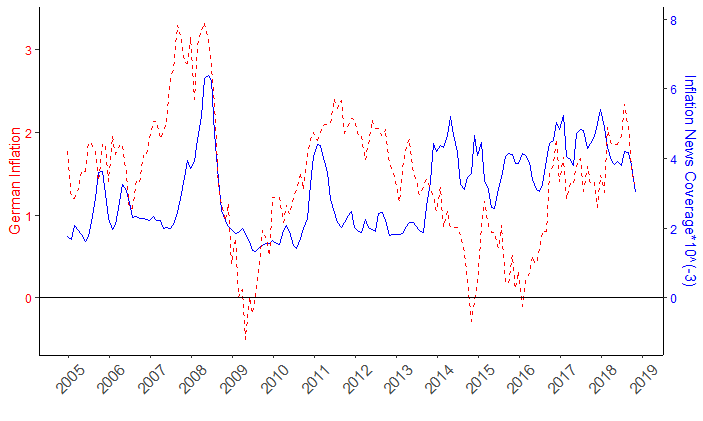
\includegraphics{Inflation_Count.png}
    \caption{Media Coverage and Inflation}
    \label{10}
\end{subfigure}
\hfil
\begin{subfigure}{6cm}
    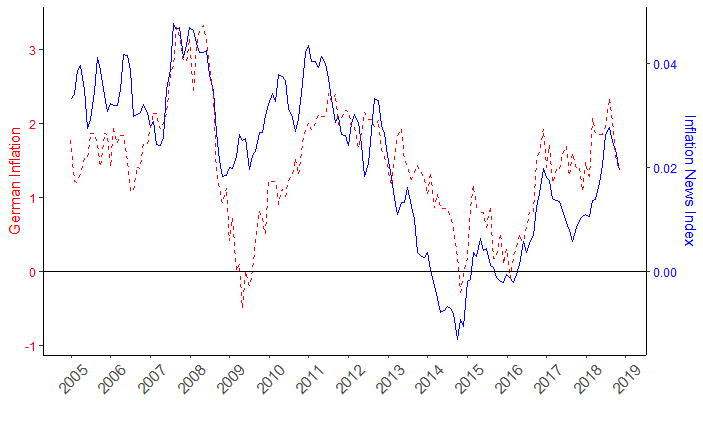
\includegraphics{Inflation_Sentiment_Direction.png}
    \caption{News Inflation Index and Inflation}
    \label{100}
\end{subfigure}
\caption{Media Reporting and Inflation. Figure (a) depicts the monthly HICP growth for Germany and the media coverage. Media Coverage is defined as inflation related sentence divided by the total number of sentences to account for the varying number of articles in each year. Figure (b) depics the monthly HICP growth for Germany and the INI.}
\label{fig:News Index}
    \end{figure}

Figure~\ref{fig:ECB Index} depicts the three ECB indezes and corresponding macroeconomic variables. 

   \begin{figure}[h!]
    \centering
    \setkeys{Gin}{width=\linewidth,height=6cm} %set image parameters
\begin{subfigure}{6cm}
    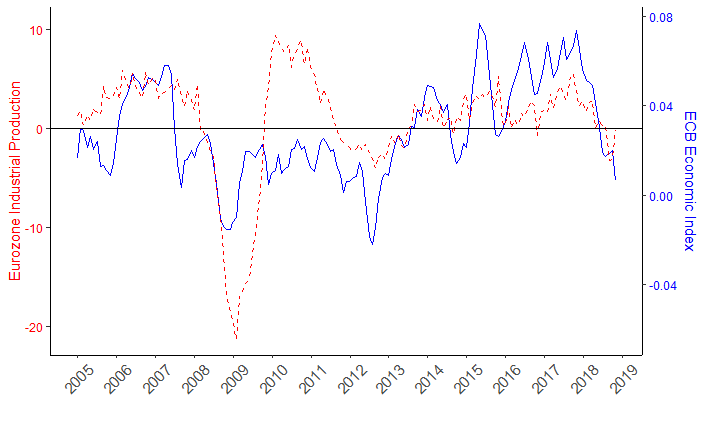
\includegraphics{ECB_eco_Industrial_prod.png}
    \caption{ECB Economic Outlook}
    \label{ECB_eco}
\end{subfigure}
\hfil
\begin{subfigure}{6cm}
    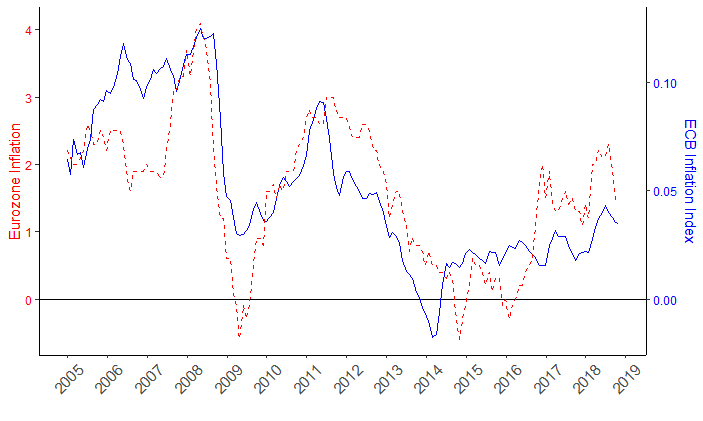
\includegraphics{ECB_inf_inf.png}
    \caption{ECB Inflation}
    \label{ECB_inf}
\end{subfigure}
\vfil
\begin{subfigure}{6cm}
    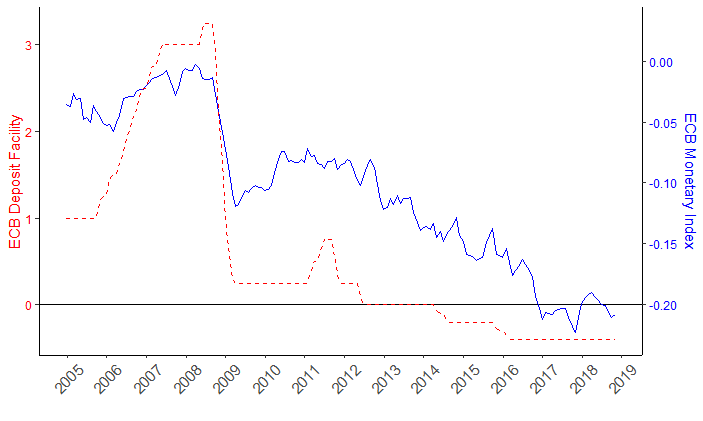
\includegraphics{ECB_mon_df.png}
    \caption{ECB Monetary}
    \label{ECB_inf}
\end{subfigure}
\caption{ECB Indices. Figure (a) depicts the monthly growth of the industrial production in the Eurzone together with the Ecoonomic Outlook index. Figure (b) depicts the monthly HICP growth for the Eurzone together with the ECB inflation outlook index. Figure (c) depicts the deposit facilitie rates together with the monetary outlook index.}
\label{fig:ECB Index}
    \end{figure}
\newpage
\textcolor{red}{NOTE 1: Professional Forecaster Inflation Expectations are stronger correlated with ECB Inflation Index than with Inflation Expectations. Could be because of the European prof. Inf. Exp.}
\\
\textcolor{red}{NOTE 2: The results are quite similar to Picault et. al (2017) and Marozzi (2021), which is reassuring, but I only add 4 more years to the dataset. Therefore, my approach adds little new information regarding the ECB indices.}

Both the relative and absolute residuals show a strong correlation until 2014. However,  

%\cite{Carroll2003} define the inflation expectation error of households as the squared difference between the household inflation expectations and professional inflation expectations. \cite{LamlaLein2014} instead uses the absolute difference. Because I'm not only interested in the absolute size of the inflation gap, but also the direction 

%To measure the error, I use the EU household inflation expectation described in and the professional inflation forecasts for the Eurozone described in (SECTION 2). My interest lies in the deviation between the household inflation expectations from the optimal forecasts. Therefore, I follow Lamla (2014) and calculate the household forecast errors as the difference between the household inflation expectations and professional inflation forecast for the Eurozone in the coming 12 months. I deviate from Lamla (2014) by taking the non-absolute error. (CITE) and (CITE) show that households react differently to news regarding high and low inflation.

\newpage

   \begin{figure}[h!]
    \centering
    \setkeys{Gin}{width=\linewidth,height=6cm} %set image parameters
\begin{subfigure}{6cm}
    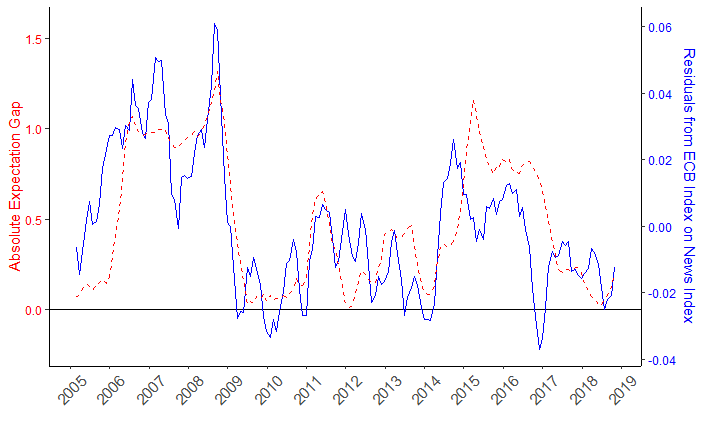
\includegraphics{abs_exp_res.png}
    \caption{Absolute Expt. Gap}
    \label{10}
\end{subfigure}
\hfil
\begin{subfigure}{6cm}
    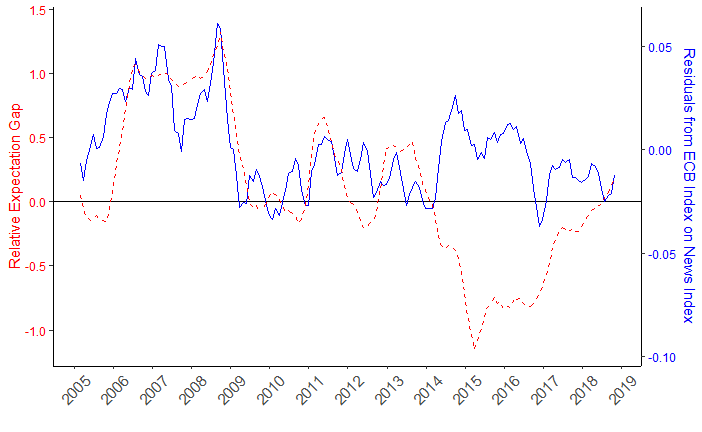
\includegraphics{rel_exp_res.png}
    \caption{Relative Expt. Gap}
    \label{100}
\end{subfigure}
\vfil
\begin{subfigure}{6cm}
    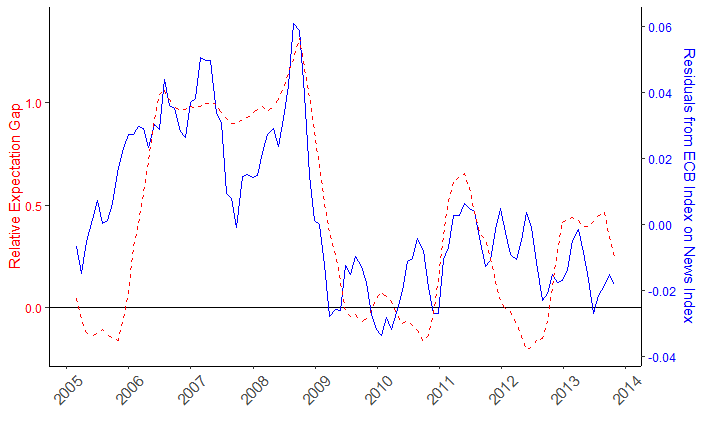
\includegraphics{rel_exp_res_prev2014.png}
    \caption{Relative Expt. Gap - Before 2014}
    \label{ECB_inf}
\end{subfigure}
\hfil
\begin{subfigure}{6cm}
    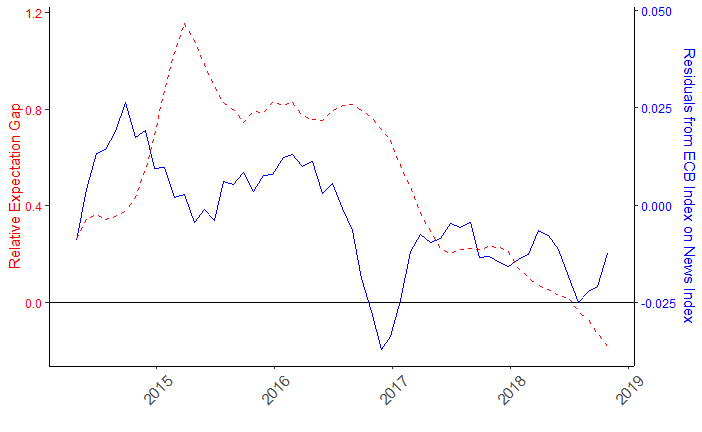
\includegraphics{rel_exp_res_aft2014.png}
    \caption{Negative Relative Expt. Gap - After 2014}
    \label{ECB_inf}
\end{subfigure}
\caption{Figure (a) shows the absolute expectation gap and regression residuals between the ECB inflation outlook and News inflation indices. Figure (b) presents the relative expectation gap and corresponding residuals. Figures (c) and (d) display the relative expectation gap for 2005-2014 and 2014-2018, respectively.}
\label{fig:Expectation Gap}
    \end{figure}

%\section{Model}\label{sec:Model}

%$\pi^i_t$ = information regarding inflation which agents follow \\
%$\pi^{ECB}_t$ = information regarding inflation from ECB \\
%$\pi^n_t$ = information regarding inflation from news \\
%
%$\epsilon_t$ = normal distributed error with mean zero and variance $\sigma_{ECB,t}$ \\
%$\gamma_t$ = media bias \\
%$\lambda_t$ = media bias weight (1 = full bias, 0 bias) \\
%
%$\pi^{ECB}_t$ = $\pi^{Eurozone}_t + \epsilon_t$ (assuming that ECB is unbiased and focused on the Eurozone as a whole instead of country specific inflation.) 
%\\
%\textcolor{red}{Check if other papers made a difference for Eurozone inflation and country specific inflation.}
%\\
%
%$\pi^n_t$ = $\lambda_t * \pi^{ECB}_t + (1-\lambda_t) * (\gamma_t + \pi_t)$ (News can either follow ECB and just reproduce the ECBs press conferences ($\lambda_t = 1)$ or they could ignore the press conferences completely ($\lambda_t = 0$).) \\

%$\pi^i_t$ = $\alpha_t * \pi^{ECB}_t + (1-\alpha_t) * \pi^n$ \\
%$\pi^i_t$ = $\alpha_t * (\pi_t + \epsilon_t) + (1-\alpha_t) * (\pi_t + \lambda_t * \pi^{ECB}_t + (1-\lambda_t) * \gamma_t)$ \\
%$\pi^i_t$ = $\pi_t + \alpha_t * \epsilon_t + (1-\alpha_t) * (\lambda_t * \pi^{ECB}_t + (1-\lambda_t) * \gamma_t)$ \\

\section{Econometric Framework}\label{sec:Econometric Framework}
To test my hypthesis 
\textcolor{red}{to close to Erhmann et al. 2017?}
\\
$\mathbf{B}_t = \alpha + \beta_1 Media^{count}_t + \beta_2 Media^i_t + \beta_3 Media^{cb}_t +\beta_3 \pi_{t-1} + \epsilon_t$ \\
where $\alpha$ is a constant, 

%$Media^c_t$ is the news count in period $t$, $Media^i_t$ is the news inflation index and Media^{cb}_t

The equation is estimated via OLS using Newey-West standard errors.
\\
To avoid simultaneity issues I follow \cite{LamlaLein2014} In order to obtain media data for a given month, I aggregate the media reports for each month, excluding any articles which are potentially related to the consumer survey results in the month. Specifically, I sum up the media articles until the day before the consumer survey is released. The sentences from the summed up articles are then used to derive the news index and news count for the given month.
\\
\textcolor{red}{Andere finden die das ähnlich gemacht haben.}
\\


\begin{table}[!h]
\centering 
  \caption{Inflation Expectation Gap} 
  \label{tab:Inflation Expectation Gap}
\begin{tabular}{l*{6}{c}}   
\toprule
 & $B^r_t$ & $B^e_t$ & $\pi_{t+1}$ & & & \\ 
\midrule
$B^r_{t-1}$ & & & & & & \\
$B^e_{t-1}$ & & & & & & \\
$NewsInflation_t$ & & & & & & \\
$ECBInflation_t$ & & & & & & \\
$ECBMonetary_t$ & & & & & & \\
$ECBOutlook_t$ & & & & & & \\
$News ECB Difference_t$ & & & & & & \\
$\pi_t$ & & & & & & \\
%$IndustrialProduction_t$ & & & & & & \\
$Constant$ & & & & & & \\
\midrule
$R^2$ & & & & & & \\
\bottomrule
 \end{tabular} 
\end{table}

\section{Results}\label{sec:Results}



\section{Conclusions} \label{sec:Conclusions}

%\section*{References}

\bibliography{mybibfile}

\newpage

\appendix

\section{Quantification of Inflation Expectations}\label{sec:Quantification of Inflation Expectations}

The European Commission's Business and Consumer Survey consumers are asked if they expect prices to fall, stay the same, increase slower than before, increase at the same rate or increase at a higher rate in the coming 12 months and in the last 12 months. 
\\
I use the rolling-window-regression approach by \cite{Lahiri2015} which is based on an extended version of the Carlson-Parkin method \citep{Carlson1975} by \cite{Berk1999}. The extended version of \cite{Berk1999} does not impose unbiasedness of inflation expectations. Instead the current perceived inflation rate is directly linked to the expected inflation rate.  
\\
By assumption each responded i forms a subjective probability distribution for individuals percentage price changes $y_{it}$ over the next twelve months. Let $f_i(y{_it})$ be the subjective probability distribution with mean $\mu_{it}$ and variance $\sigma_{it}$. Following \cite{Batchelor1988} method assumes for a survey with five possible answers that the respondent answers prices in the future increase, increase at the same rate, increase at a slower rate, stay the same or fall according as $ y_{it} < - \delta_{it}^L, - \delta_{it}^L < y_{it} < \delta_{it}^U , \delta_{it}^L < y_{it} < \delta_{it}^U,  \delta_{it}^U < y_{it} < \lambda_{it}, \lambda_{it} < y_{it}$ \textcolor{red}{Nochmal überprüfen, Ist Notation von \cite{Batchelor1988} besser?}. Based on the survey responses the corresponding aggregate probabilities can be formulated as $P(y <  -\delta_{it}^L) = A_t, P(y < \delta_{it}^U) - P(y > - \delta_{it}^L) = B_t, P(y < \delta_{it}^U) - P(y > \delta_{it}^L) = C_t, P(y < \lambda_{it}) - P(y > \delta_{it}^U) = D_t.$ I denote $a_t, b_t, c_t$ and $ d_t$ the abscissae of the standard logistical distribution function corresponding to the cumulative probabilities $A_t, \ A_t + B_t, \ A_t + B_t + C_t$ and $A_t + B_t + C_t + D_t$. The mean expected inflation rate $\mu_t = E_t \pi_{t+12}$ can then be formulated as 
\begin{align*}
\mu_t = \lambda_t \frac{(a_t + b_t)}{(a_t + b_t - c_t - d_t)}
\end{align*}
Similarly, I denote $a_t\sp{\prime}, b_t\sp{\prime}, c_t\sp{\prime}$ and $ d_t\sp{\prime}$ as the abscissae of the standard logistical distribution function for the perceived inflation. Assuming that the response threshold $\lambda_{it}$ \textcolor{red}{Nochmal überprüfen} is the same for expected and perceived inflation, the perceived inflation can be formulated as 
\begin{align*}
\mu_t\sp{\prime} = \lambda_t \frac{(a_t\sp{\prime} + b_t\sp{\prime})}{(a_t\sp{\prime} + b_t\sp{\prime} - c_t\sp{\prime} - d_t\sp{\prime})}
\end{align*}
For the choice of the scaling parameter $\lambda_t$ I use the rolling window based regression by \cite{Lahiri2015}. Following \cite{Rosenblatt-Wisch2015} running the regression
\begin{align*}
\pi_t = \lambda \frac{(a_t\sp{\prime} + b_t\sp{\prime})}{(a_t\sp{\prime} + b_t\sp{\prime} - c_t\sp{\prime} - d_t\sp{\prime})} + u_t 
\end{align*}
using a sample window of $t - w + 1 to t$ implies
\begin{align*}
\hat{\lambda_t} = \frac{\sum^t_{k = t-w+1}(a_t\sp{\prime} + b_t\sp{\prime})/(a_t\sp{\prime} + b_t\sp{\prime} - c_t\sp{\prime} - d_t\sp{\prime})\pi_t}{\sum^t_{k = t-w+1}(a_t\sp{\prime} + b_t\sp{\prime})/((a_t\sp{\prime} + b_t\sp{\prime} - c_t\sp{\prime} - d_t\sp{\prime}))^2}
\end{align*}
where $w$ is the size of the rolling window. \cite{Lahiri2015} choose $w$ as nine years for the inflation expectations of the Michigan Consumer Survey. I follow \cite{Lahiri2015} and also choose nine years for $w$. The resulting household inflation expectations and the professional inflation expectations are shown in figure~\ref{fig:Inflation Expectations}.
\\
\textcolor{red}{Robustness Check for different windows?}
\\
\textcolor{red}{TO CLOSE TO Rosenblatt-Wisch and Scheufele 2014??}

  \begin{figure}[h!]
    \centering
    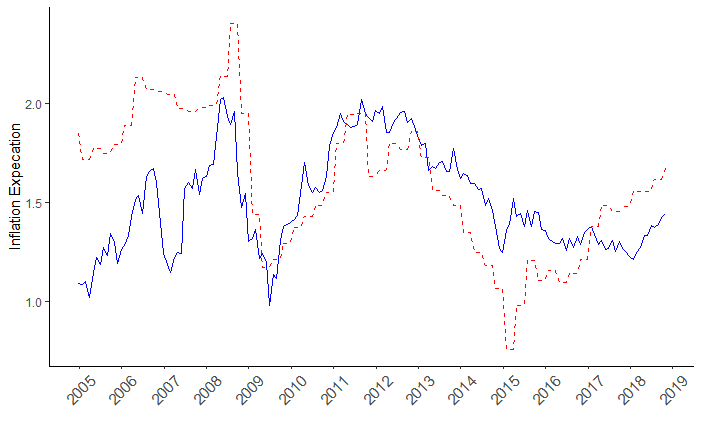
\includegraphics{household_prof_inf.png}
    \caption{Inflation Expectations: Household inflation expectations are in blue, Professional forecaster inflation expectations are in red}
    \end{figure}
\label{fig:Inflation Expectations}

\section{Additional Rules for Lexicon Text Classification}\label{sec:Additional Rules for Lexicon Text Classification}

\end{document}